\documentclass
%[handout]
{beamer}
%\documentclass{beamer}

%%
%%
%%
% From http://tex.stackexchange.com/questions/2072/beamer-navigation-circles-without-subsections
% Solution #2 or 3:
% \usepackage{etoolbox}
% \makeatletter
% % replace the subsection number test with a test that always returns true
% \patchcmd{\slideentry}{\ifnum#2>0}{\ifnum2>0}{}{\@error{unable to patch}}%
% \makeatother
% Solution #1:
\usepackage{remreset}% tiny package containing just the \@removefromreset command
\makeatletter
\@removefromreset{subsection}{section}
\makeatother
\setcounter{subsection}{1}


\usepackage{etex}
\usepackage{pgf}
\usepackage{tikz}
\usepackage{url}
\usepackage{amsmath}
\usepackage{color}
% \definecolor{red}{rgb}{1,0,0}
\usepackage{ulem}
% \usepackage{booktabs}
\usepackage{colortbl,booktabs}
\renewcommand*{\thefootnote}{\fnsymbol{footnote}}
\usepackage{fancybox}
\usepackage[framemethod=TikZ]{mdframed}
\mdfdefinestyle{FactStyle}{%
  outerlinewidth=0.5,
  roundcorner=1pt,
  leftmargin=1cm,
  linecolor=blue,
  outerlinecolor=blue!70!black,
  backgroundcolor=yellow!40
}
\usepackage{cancel}

  \newcommand\Warning{%
    \makebox[2.4em][c]{%
      \makebox[0pt][c]{\raisebox{.2em}{\Large!}}%
      \makebox[0pt][c]{\color{red}\Huge$\bigtriangleup$}}}%

\usepackage{stackengine}
\usepackage{scalerel}
\usepackage{xcolor}
  \newcommand\dangersign[1][2ex]{%
    \renewcommand\stacktype{L}%
    \scaleto{\stackon[1.3pt]{\color{red}$\triangle$}{\tiny !}}{#1}%
  }



\usepackage{dcolumn}
\newcolumntype{d}[1]{D{.}{.}{#1}}

% From
% http://tex.stackexchange.com/questions/109900/how-can-i-box-multiple-aligned-equations
\usepackage{empheq}
\usepackage{tcolorbox}  \newtcbox{\othermathbox}[1][]{%
  nobeforeafter, tcbox raise base, 
  colback=black!10, colframe=red!30, 
  left=1em, top=0.5em, right=1em, bottom=0.5em}

\newcommand\blue{\color{blue}}
\newcommand\red{\color{red}}
\newcommand\green{\color{green!75!black}}
\newcommand\purple{\color{purple}}
\newcommand\bluegreen{\color{blue!75!green}}
\newcommand\orange{\color{orange}}
\newcommand\redgreen{\color{red!50!green}}
\newcommand\grey{\color{black}}
\newcommand\gap{\vspace{.1in}}
\newcommand\nb{${\red\bullet}\ $}
\newcommand\halfgap{\vspace{.05in}}
\newcommand\divideline{\line(1,0){352}}
\usepackage{marvosym} % for \Smiley

\newcommand{\bluealert}[1]{{\blue\textbf{#1}}}

% \usepackage{beamerthemesplit} %Key package for beamer
\usetheme{Singapore}
% \usetheme{Szeged}
% \usetheme{Garfield}
% \usetheme{CambridgeUS}
% \usenavigationsymbolstemplate{} %Gets rid of slide navigation symbols


\setbeamercolor{separation line}{use=structure,bg=structure.fg!50!bg}
% \begin{beamercolorbox}[colsep=0.5pt]
%   {upper separation line foot}
% \end{beamercolorbox}



\makeatletter
\setbeamertemplate{footline}
{
  \leavevmode%
  \hbox{%
% \begin{beamercolorbox}[colsep=0.5pt]
%   {upper separation line foot}
% \end{beamercolorbox}


  \begin{beamercolorbox}[wd=.5\paperwidth,ht=2.25ex,dp=2ex,colsep=0.5pt]%
    {upper separation line foot}
    \usebeamerfont{author in head/foot}%
    \hspace*{2ex}\insertshortdate:\ \insertshorttitle
  \end{beamercolorbox}%
  \begin{beamercolorbox}[wd=.5\paperwidth,ht=2.25ex,dp=2ex,right]{title in head/foot}%
    \usebeamerfont{title in head/foot}
    {\insertshortauthor}\hspace*{2ex}
  \end{beamercolorbox}}%
  % \begin{beamercolorbox}[wd=.333333\paperwidth,ht=2.25ex,dp=2ex,right]{date in head/foot}%
  %   \usebeamerfont{date in head/foot}\insertshortdate{}\hspace*{2em}
  %   \insertframenumber{} / \inserttotalframenumber\hspace*{2ex} 
  % \end{beamercolorbox}%
  \vskip0pt%
}
\makeatother

\usetikzlibrary{decorations.markings}
\usetikzlibrary{arrows}


\title{Final Exam Review}
\author{Peter Garfield, UCSB Mathematics}
\date{March 15, 2017}
%\institute{}


\useinnertheme{default}

\usefonttheme{serif}
% \usecolortheme{rose}
% \usecolortheme{whale}
% \usecolortheme{orchid}
\usecolortheme{crane}
% \usecolortheme{dolphin}


%TEMPLATE
\setbeamertemplate{navigation symbols}{}

\setbeamertemplate{note page}[compress]

\setbeamertemplate{frametitle}{
  \vspace{0.5em}
  % \begin{centering}
  {\huge\blue\textbf{\textmd{\insertframetitle}}}
  \par
  % \end{centering}
}

% From http://tex.stackexchange.com/questions/7032/good-way-to-make-textcircled-numbers:
\newcommand*\circled[1]{\tikz[baseline=(char.base)]{\node[shape=circle,draw,fill=orange,inner sep=1pt] (char) {#1};}} 
% \renewcommand{\labelenumi}{\circled{\textbf{\arabic{enumi}}}}

\let\olddescription\description
\let\oldenddescription\enddescription
\usepackage{enumitem}
\let\description\olddescription
\let\enddescription\oldenddescription

% \usepackage[loadonly]{enumitem}
\setlist[enumerate,1]{label=\colorbox{orange}{\arabic*.},font=\bfseries}
%\setlist[enumerate,2]{label=\colorbox{blue!25}{(\alph*)},font=\bfseries}
% \setlist[enumerate,1]{label=\arabic*.,font=\bfseries}
\setlist[itemize,1]{label=\red$\bullet$}
\setlist[itemize,2]{label=\blue$\bullet$}

\newcommand\answer[1]{\fbox{#1}}
% \renewcommand\answer[1]{}

\newcommand{\antilog}{\operatorname{antilog}}








\title{}
\title{Calculus Intro}
\date{May 3, 2022}


\begin{document}
\small



\section*{Administration}

\frame{
  \frametitle{}
  {\Huge{}Welcome Back!}\\[.5em]

  {\Huge{}Differential Calculus}
  \vfill
  {\Large{}Instructor:}\\
  \ \hspace*{0.2in} Nathan Schley ({\it Sh}+{\it lye}), \url{schley@math.ucsb.edu}\\
  \ \hspace*{0.2in} South Hall 6701
  \\[0.5em]

  {\Large{}Office Hours:}\\
  \ \hspace*{0.2in} T R 11-11:50, T 3:45-4:35 Details on Gauchospace. 
  \bigskip

  \copyright\ 2022\ Daryl Cooper, Peter M.\ Garfield, Ebrahim Ebrahim \& Nathan Schley\\
  Please do not distribute outside of this course.
  \vfill

}




% \frame{
%   \frametitle{i-clicker}

%   {\large {\blue If you have been having i-clicker trouble, please email me about this with a photo of your i-clicker and your Gauchospace page. The first photo gives ID the serial number for your i-clicker and the second verifies your identity (for them). } }
  
  
  

% } 

\frame{
  \frametitle{Warm-up}

  {\large {\blue } }
  \begin{itemize} 
  \item $\log(x) =5$ \ \ \ \ \ \ \ \ \ \  \pause  $x=$\fbox{$10^5$} \pause = \fbox{$100,000$}
  \pause
  \item $10^x = 1,000,000$ \pause \ \ $x=$\fbox{$\log(10^6)$} \pause = \fbox{$6$}
  \pause
  \item $\log(\log(x)) =2$ \ \ \ \  \pause  $x=$\fbox{$10^{10^2}$} \pause = \fbox{$10^{100}$}
  \pause
  \item $10^x = 2$ \pause \ \ \ \ \ \ \ \ \ \ \ \ \ \ $x=$\fbox{$\log(2)$} \pause {\blue $\approx$ \fbox{$.3$}}
  \pause
  \item $10^x = 8700$ \pause \ \ \ \ \ \ \ \ \ \ \ $x=$\fbox{$\log(8700)$} \pause {\blue $\approx$ ?}\pause \\
  $8700 = 8.7\cdot10^3$ \ \ \ \  \pause {\blue $\log(8700) = \log(8.7) + 3$}
  \pause
  \item $10^{4x-5} = 7$ \pause \ \ \ \ \ \ \ \ $x=$\fbox{$(\log(7)+5)/4$} \pause {\blue $\approx$ \fbox{?} \pause just leave it that way}
  %\pause
  %\item $7^{4x-5} = 7$ \pause \ \ \ \ \ \ \ \ \ $x=$\fbox{$(1+5)/4$} \pause = \fbox{$3/2$} 
  
  
  \end{itemize}
  
  
  

} 

\frame{
  \frametitle{Logarithm Strategy}

  
  \begin{itemize} 
  \item $4^{2x+1} = 3$ \pause \ \ \ \ \ \ \ \ $x=$\fbox{$(\log_4(3)-1)/2$} \pause $= (\frac{\log(3)}{\log(4)} - 1)/2$ \vspace{20pt} \\
  {\large {\blue In general, \\ \centerline{\fbox{$\log_b(x) = \frac{\log(x)}{\log(b)}$}} } }
  
  \end{itemize}
  
  
  

} 

\section*{Exam Info}

\frame{
  \frametitle{Midterm 2: One week from today}

  {\Large\color{blue}Bring:}
  \begin{itemize}
  \item A pen or \alert{sharp} pencil. 
  \item A $3"\times5"$ card with your notes. 
  \item Student ID. 
  \end{itemize}
  \bigskip

  {\Large\color{red}Don't bring:}
  \begin{itemize}
  \item A calculator
  \end{itemize}
  \smallskip

  No bluebook or scratch paper necessary, just the above materials and hopefully a fresh, well-practiced you! Scratch paper will be provided. 

}


\frame{
  \frametitle{Midterm 2 Topics}

  \begin{itemize}
  \item All topics from Midterm 1
  \item Sums (like the example below, more examples on Gauchospace)
  $$\sum_{n=1}^{4} 2^n-1$$
  \item Advanced Logarithm Methods (the full chapter on logarithms in the book)
  \item Change and Average Rate of Change for a function or graph. 
  \item Limits with $h$ (used to find exact speed, examples on the old midterm and extra problems)
  \end{itemize}

  \smallskip

  If you struggled on Midterm 1 with algebra or word problems, you need to improve these skills immediately. {\bf They are essential for success in this course}. 

}


\section*{Rate of Change}

\frame{
  \frametitle{Graphical Approach}

  \begin{minipage}{0.5\linewidth}
    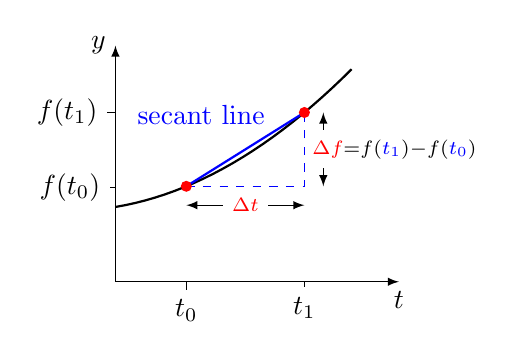
\begin{tikzpicture}[x=12mm,y=12mm,>=latex]
        \draw[black,->] (0,0) -- (3,0) node[below] {$t$};
        \draw[black,->] (0,0) -- (0,2.5) node[left] {$y$};
        % Ticks:
        \draw[thin,black] (0.75,0) -- (0.75,-3pt) node[below] {$t_0$};
        \draw[thin,black] (2,0) -- (2,-2pt) node[below] {$t_1$};
        \draw[thin,black] (0,1) -- (-2pt,1) node[left] {$f(t_0)$};
        \draw[thin,black] (0,{0.75+(2+1/2)^2/6}) -- (-3pt,{0.75+(2+1/2)^2/6}) node[left] {$f(t_1)$};
        \draw[black,thick] plot[domain=0:2.5] (\x,{0.75+(\x+1/2)^2/6});
      %
        \draw[thick,blue] (0.75,{0.75+(0.75+1/2)^2/6}) -- (2,{0.75+(2+1/2)^2/6}) node[near end,left,yshift=2mm] {secant line};
        \draw[thin,black,<->] (0.75,{0.75+(0.75+1/2)^2/6-0.2}) -- (2,{0.75+(0.75+1/2)^2/6-0.2}) node[midway,red,fill=white] {$\scriptstyle\Delta t$};
        \draw[thin,black,<->] (2.2,{0.75+(0.75+1/2)^2/6}) -- (2.2,{0.75+(2+1/2)^2/6}) node[midway,fill=white,right,xshift=-0.75em] {$\scriptstyle{\red\Delta f}=f({\blue t_1})-f({\blue t_0})$};
        \draw[thin,blue,dashed] (0.75,{0.75+(0.75+1/2)^2/6}) -- (2,{0.75+(0.75+1/2)^2/6}) -- (2,{0.75+(2+1/2)^2/6});
        % 
      %
        \fill[red] (0.75,{0.75+(0.75+1/2)^2/6}) circle (2pt);
        \fill[red] (2,{0.75+(2+1/2)^2/6}) circle (2pt);
    \end{tikzpicture}
  \end{minipage}
  \hfill
  \parbox{50mm}{%
    ${\red\Delta f}=$ change in $f$ \\
    ${\red\Delta t}=$ change in $t$\\[0.5em]
    \alert{Many ways to say same thing:}\\
    $\begin{array}{l}
       \left(\begin{array}{c} \text{{\blue average} rate of}\\ \text{change of $f$}\end{array}\right)  = \dfrac{\text{change in $f$}}{\text{change in $t$}}\\
       = \dfrac{\red \Delta f}{\red\Delta t}\\
       =  \text{slope of {\blue secant line}}
       = \dfrac{f({\blue t_1})-f({\blue t_0})}{{\blue t_1}-{\blue t_0}}
     \end{array}$
   }
   \pause

   The derivative is defined to be
   \begin{equation*}
     \lim_{\Delta t\to0} \left(\frac{\red\Delta f}{\red\Delta t}\right) 
     = \frac{df}{dt}
   \end{equation*}
   \pause

   Idea: As $t_1$ moves closer to $t_0$ the secant line approaches the {\blue tangent line}  at $t_0$.
   This is the line with the {\blue same slope} as the graph at $t_0$.

   % \fbox{{\red Let's watch a movie }} \qquad\qquad  No, not  {\blue The Bourne Identity}  :(\\

   % http://www.youtube.com/watch?v=AdQG2iSLDjA\\
   % http://www.youtube.com/watch?v=s3q8D79bjiE\&feature=related
}


\frame{
  \frametitle{Understanding Derivatives}

  There are many ways to {\blue think} about derivatives.  We {\blue
    need} to understand how derivatives apply to problems. 
  \gap
  \gap 

  \begin{minipage}{0.35\linewidth}
    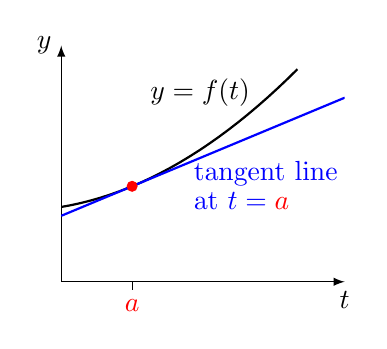
\begin{tikzpicture}[x=12mm,y=12mm,>=latex]
        \draw[black,->] (0,0) -- (3,0) node[below] {$t$};
        \draw[black,->] (0,0) -- (0,2.5) node[left] {$y$};
        % Ticks:
        \draw[thin,black] (0.75,0) -- (0.75,-3pt) node[below] {\red$a$};
        % \draw[thin,black] (2,0) -- (2,-2pt) node[below] {$t_1$};
        % \draw[thin,black] (0,1) -- (-2pt,1) node[left] {$f(t_0)$};
        % \draw[thin,black] (0,{0.75+(2+1/2)^2/6}) -- (-3pt,{0.75+(2+1/2)^2/6}) node[left] {$f(t_1)$};
        \draw[black,thick] plot[domain=0:2.5] (\x,{0.75+(\x+1/2)^2/6});
        \begin{scope}
          \clip (0,0) rectangle (3,2.5);
          \draw[blue,thick] plot[domain=0:3] (\x,{(0.75+1/2)*(\x-0.75)/3+0.75+(0.75+1/2)^2/6});
          \node[blue,right] at (1.3,1.15) {tangent line};
          \node[blue,right] at (1.3,0.85) {at $t={\red{}a}$};
          \node[left] at (2.1,2) {$y=f(t)$};
        \end{scope}
      %
      %
        \fill[red] (0.75,{0.75+(0.75+1/2)^2/6}) circle (2pt);
    \end{tikzpicture}
  \end{minipage}
  \hfill
  \parbox{60mm}{%
    slope of {\blue graph} at {\red a}\\
    = slope of {\blue tangent line} \\%\small{\red $\quad\quad^{discuss}$}\\
    = {\purple instantaneous rate of change} of $f$ at ${\red a}$\\
    \\
    $= \left(
      \begin{array}{l}
        \text{limit of average rate of change } \\ 
        \text{of $f$ over shorter and shorter}\\
        \text{ time intervals starting at\ {\red$a$}}
      \end{array}
    \right)$\\
    \\
    $=$ limit of slopes of secant lines\\
    $= f'({\red a})\ =\ \left. \dfrac{df}{dt}\right|_{t={\red a}}$
  }

}

\frame{
  \frametitle{Summary}

  \begin{itemize}
  \item[$\red \bullet$] How fast something changes $=$ {\blue rate of
      change}
    \bigskip

  \item[$\red \bullet$] {\red Instantaneous} {\blue rate of change} is
    the {\redgreen limit} of the average rate of change over shorter
    and shorter time spans. This gets around the changing speed problem, and works a whole lot better that getting frustrated and trying ${\red 0/0}$. 
    \bigskip

  \item[$\red \bullet$] {\blue speed} $=$ rate of change of distance traveled.
    \bigskip

  \end{itemize}

}

\frame{
  \frametitle{Speed=Slope=Derivative}
  \begin{minipage}{0.5\linewidth}
    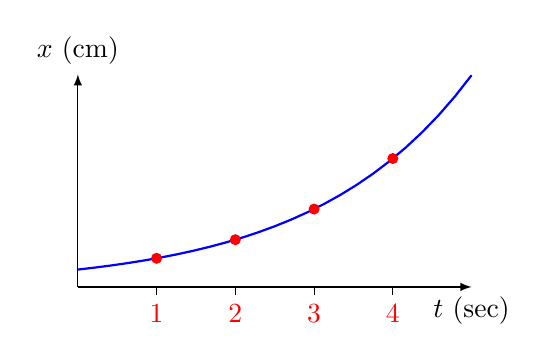
\begin{tikzpicture}[x=10mm,y=6mm,>=latex]
      \draw[thin,black,->] (0,0) -- (5,0) node[below] {$t$ (sec)};
      \draw[thin,black,->] (0,0) -- (0,4.5) node[above] {$x$ (cm)};
      \draw[thick,blue] plot[domain=0:5] (\x,{exp((\x-2)/2)});
      \foreach \x in {1,2,3,4}
      {
        \draw[thin,black] (\x,0) -- (\x,-3pt) node[below] {$\red\x$};
        \fill[red] (\x,{exp((\x-2)/2)}) circle (2pt);
      }
    \end{tikzpicture}
  \end{minipage}
  \hfill
  \begin{minipage}{0.4\linewidth}
    The graph shows the distance from the origin in cm after $t$
    seconds of a hamster.  Which of the numbers below is the largest? 
    \bigskip
    
    \textbf{Hint:}\ Speed is a slope!
  \end{minipage}

  \begin{align*}
    \text{A} & = \text{speed of the hamster at $t=1$} \\
    \text{B} & = \text{speed of the hamster at $t=2$} \\
    \text{C} & = \text{speed of the hamster at $t=3$} \\
    \text{D} & = \text{average speed of the hamster between $t=2$ and $t=3$} \\
    \text{E} & = \text{average speed of the hamster between $t=3$ and $t=4$}
  \end{align*}
  \pause
  \alert{Answer:}\ \fbox{E}

}

\frame{
  \frametitle{Practical Meaning}

  Our goal is that you understand the {\blue practical meaning} of the
  derivative in various situations. 
  \gap
  \pause

  \begin{align*}
    f({\blue t})
    & = \text{temperature in ${}^{\circ}\ \text{F}$ at ${\blue t}$ hours after midnight}\\
    f({\blue 7})
    & = {\orange 48}\ 
      \text{means the temperature at {\blue 7}am was ${\orange 48}^\circ\ \text{F}$}\\
    f{\red '}({\blue 7})
    & ={\orange 3}\ 
      \text{means}\
      \text{at {\blue 7}am the temperature was rising at a rate of
      ${\orange 3}^{\circ}\ \text{F}/\text{hr}$} \\
    f{\red '}({\blue 9})
    & ={\orange -5}\ 
      \text{means}\ 
      \text{at {\blue 9}am the temperature was {\red falling} at a
      rate of ${\orange 5}^{\circ}\ \text{F}/\text{hr}$}\\ 
    & \hspace*{0.75in}\text{or {\red rising} at a rate of ${\orange
      -5}^{\circ}\ \text{F}/\text{hr}$}
  \end{align*}
  \gap
  \pause
  \begin{align*}
    g({\blue t})
    & = \text{distance from origin in cm of hamster on $x$-axis  after $\blue t$ seconds}\\
    g({\blue 7})
    & ={\orange 3}\
      \text{means after ${\blue 7}$ seconds hamster was ${\orange 3}$ cm from origin}\\
    g{\red '}({\blue 9})
    & ={\orange -5}\
    \text{means after {\blue 9} seconds our furry friend was running {\blue towards}}\\ 
    & \hspace*{0.25in}\text{the origin at a speed of ${\orange 5}\ \text{cm}/\text{sec}$}
  \end{align*}
}

\frame{
  \frametitle{Another Context}
  
  Suppose $f({\blue t})=$ temperature of oven in ${}^{\circ} \text{C}$
  after $t$ minutes.
  \smallskip

  What do $f(3)=20$ and $f{\red '}(3)=15$ mean?
  \begin{itemize}
  \item[A] After $20$ minutes the oven was at $3^{\circ}\ \text{C}$ and heating up at a rate of $15^{\circ}\ \text{C}/\text{min}$

  \item[B] After $3$ minutes oven temperature was $15^{\circ}\ \text{C}$ and cooling down at a rate to $20^{\circ}\ \text{C}/\text{min}$ 

  \item[C] The oven was heating up at rate of $3^{\circ}\ \text{C}/\text{min}$ after 15 minutes and also after 20 minutes

  \item[D] After 3 minutes the oven was at $20^{\circ}\ \text{C}$ and heating up at a rate of $15^{\circ}\ \text{C}/\text{min}$ 

  \item[E] None of the above

  \end{itemize}
  \pause
  \alert{Answer:}\ \fbox{D}

}

\section*{Derivatives in Context}

\frame{
  \frametitle{Context: Population}

  Suppose $f(t)=$ the population of the ancient city of Lyrad in
  year $t$.  %{\blue C.E.} = {\blue C}urrent {\blue E}ra
  We are told that  $f(1550) = 1820$ and $f{\red '}(1650) = 1100$.
  Which of the following is true?

  \begin{itemize}
  \item[A] In 1550, the population was 1820 and rising at a rate of 1100 people per year

  \item[B] In 1650, the population was 1100 more than in 1550

  \item[C] In 1650, Lyrad contained 1100 people

  \item[D] In 1550, there were 1820 people in Lyrad, and by 1650 this had increased to 2920

  \item[E] None of above
  \end{itemize}
  \pause

  \alert{Answer:}\ \fbox{E}
}


\frame{
  \frametitle{Context: Mathematics}

  Suppose $f(0)=50$ and $f(10)=70$.  Which of the following is true?

  \begin{itemize}
  \item[A] For all $t$ between $0$ and $10$, the derivative is $f{\red'}(t)=2$

  \item[B] $f{\red'}(0)=2$

  \item[C] It is possible that $f{\red'}(0)=-8$

  \item[D] It is impossible that $f{\red'}(0)=-8$

  \item[E] None of above

  \end{itemize}
  \pause
  \alert{Answer:}\ \fbox{C}
  \gap 
  \pause

  We'll see later that, for example, that $f(x)=x^2-8x+50$ has $f(0)=50$,
  $f(10)=70$, and $f{\red '}(0)=-8$. 

}

\frame{
  \frametitle{It doesn't have to be about time!}

  \begin{minipage}{0.4\linewidth}
    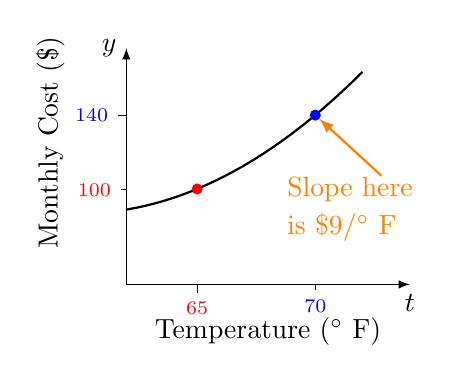
\begin{tikzpicture}[x=12mm,y=12mm,>=latex]
      \draw[black,->] (0,0) -- (3,0) node[below] {$t$};
      \draw[black,->] (0,0) -- (0,2.5) node[left] {$y$};
      % Ticks:
      \draw[thin,black] (0.75,0) -- (0.75,-3pt) node[below,red] {$\scriptstyle65$};
      \draw[thin,black] (2,0) -- (2,-2pt) node[below,blue] {$\scriptstyle70$};
      \draw[thin,black] (0,1) -- (-2pt,1) node[left,red] {$\scriptstyle100$};
      \draw[thin,black] (0,{0.75+(2+1/2)^2/6}) -- (-3pt,{0.75+(2+1/2)^2/6}) node[left,blue] {$\scriptstyle140$};
      \draw[black,thick] plot[domain=0:2.5] (\x,{0.75+(\x+1/2)^2/6});
      % 
      % \draw[thick,blue] (0.75,{0.75+(0.75+1/2)^2/6}) -- (2,{0.75+(2+1/2)^2/6}) node[near end,left,yshift=2mm] {secant line};
      % \draw[thin,black,<->] (0.75,{0.75+(0.75+1/2)^2/6-0.2}) -- (2,{0.75+(0.75+1/2)^2/6-0.2}) node[midway,red,fill=white] {$\scriptstyle\Delta t$};
      % \draw[thin,black,<->] (2.2,{0.75+(0.75+1/2)^2/6}) -- (2.2,{0.75+(2+1/2)^2/6}) node[midway,fill=white,right,xshift=-0.75em] {$\scriptstyle{\red\Delta f}=f({\blue t_1})-f({\blue t_0})$};
      % \draw[thin,blue,dashed] (0.75,{0.75+(0.75+1/2)^2/6}) -- (2,{0.75+(0.75+1/2)^2/6}) -- (2,{0.75+(2+1/2)^2/6});
      % 
      % 
      \fill[red] (0.75,{0.75+(0.75+1/2)^2/6}) circle (2pt);
      \fill[blue] (2,{0.75+(2+1/2)^2/6}) circle (2pt);
      \node[rotate=90] at (-0.8,1.5) {Monthly Cost (\$)};
      \node at (1.5,-0.5) {Temperature (${}^{\circ}\ \text{F}$)};
      \node[right,orange] at (1.6,1) {Slope here};
      \node[right,orange] at (1.6,0.6) {is $\$9/{}^{\circ}\ \text{F}$};
      \draw[thick,->,orange,shorten >=2pt] (2.7,1.15) -- (2,{0.75+(2+1/2)^2/6});
    \end{tikzpicture}
  \end{minipage}
  \hfill
  \begin{minipage}{55mm}
    $f(x) =$ monthly cost of heating house to $x^{\circ}\ \text{F}$
    \gap

    $f(70)=140$ means {\blue it costs \$140 to heat the house for one
      month to a temperature of $70^{\circ} \text{F}$.} 
    \pause
    \gap 

    ${\orange f'(70)=9}$ means {\blue {\red rate} at which cost increases
      as temperature changes is \$9 for each extra ${}^{\circ}\
      \text{F}$.}
  \end{minipage}
\pause
\gap 

In {\purple practical} terms this means {\blue you pay an extra \$9 during each month for each extra
$1^oF$}  . If you turn it up two degrees you pay an extra \$18 each
month. {\purple Each extra degree of warmth costs an extra \$9 each
  month.} 
In economics this is called a {\red marginal cost} or {\red marginal
  rate} \pause 
\gap 

This is not {\red exactly} true:\\  \qquad {\blue average} rate of
change versus {\blue instantaneous} rate of change.\\  In the
following examples we will ignore this subtlety. 


}




\frame{
  \frametitle{Get Pumped!}

  Adrenaline cause the heart to speed up.\\
  ${\blue x}=$ {\blue number of mg} (milligrams) of adrenaline in the blood.\\
  $f({\blue x})=$ {\orange number of beats per minute} (bpm) of the heart
  with ${\blue x}$ mg of adrenaline in the blood. 
  \gap

  What does $f{\red '}({\blue 5})={\orange 2}$ mean?
  \hfill\uncover<2->{\alert{Answer:}\ \fbox{E}}
  \begin{itemize}
  \item[A] When there are {\blue 5} mg of adrenaline the heart beats
    at {\orange 2} pbm

  \item[B] When the amount of adrenaline is increased by {\orange 2} mg
    the heart speeds up by {\blue 5} bpm

  \item[C] When the heart beats at {\blue 5} bpm the adrenaline is
    increased by {\orange 2} mg
 
  \item[D] When there are {\blue 5} mg of adrenaline the heart speeds
    up by {\orange 2}bpm
    
  \item[E] When there are {\blue 5} mg of adrenaline in the blood the
    heart speeds up by {\orange 2} bpm for each extra mg of adrenaline. 

  \end{itemize}
  \gap
  \textbf{Hint:}\ The {\purple units} of $ f{\red'}({\blue 5})$ are {\purple bpm per milligram of adrenaline}

}





\frame{
  \frametitle{Summary of Derivatives}

  One quantity, $\red y$, depends on another quantity $\blue x$. \\
  In other words $\red y$ is a {\blue function} of $\blue x$ so ${\red y}=f({\blue x})$.
  \hfill 
  \alert{Example:} ${\red y}={\orange 7}{\blue x}$
  \pause
  \gap

  If you change ${\blue x}$, then ${\red y}$ changes.

  \alert{Question:}\ How quickly does ${\red y}$ change as ${\blue x}$ changes? 
  \pause
  \gap

  Answer: The {\orange derivative} tells you. 
  \pause
  \gap 

  In our example, the derivative is $\orange 7$.  This tells you:
  \halfgap  

  \begin{center}
    {the {\red  output = $y$} of the function changes\\ 
      $\orange 7$ {\purple times} as fast\\ 
      as the {\blue input = $x$ } to the function.}
  \end{center}
  \gap
  \pause 

  If $\blue x$ is changed by $\blue 0.1$ how much does $\red y$ change by?
  \begin{center}
    A$=7$
    \quad 
    B$=7.1$
    \quad 
    C$=0.7$
    \quad 
    D$=0.1/7$
    \quad 
    E$=\text{other}$
    \quad
    \pause
    \fbox{C}
  \end{center}
}


\section{Interpreting Derivatives}

\frame{
  \frametitle{Graphical Meaning}

  \begin{minipage}{0.45\linewidth}
    \begin{empheq}[box=\othermathbox]{align*}
      \Large%
      \frac{d}{dx}\left( x^2\right) = 2x      
    \end{empheq}
    % \vspace{.1in}

    What this {\blue means}
    %% \vspace{.1in}

    \begin{empheq}[box=\othermathbox]{align*}
      \text{The {\red slope} of the graph\ }\\
      \text{of ${\blue y=x^2}$ at $x={\red a}$ is $2{\red a}$}
    \end{empheq}
  \end{minipage}
  \hspace*{0.25in}
  \begin{minipage}{0.45\linewidth}
    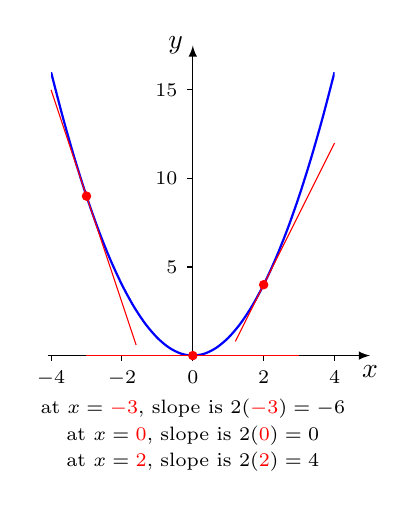
\begin{tikzpicture}[x=4.5mm,y=2.25mm,>=latex]
      \draw[thin,black,->] (-4.1,0) -- (5,0) node[below] {$x$};
      \draw[thin,black,->] (0,0) -- (0,17.5) node[left] {$y$};
      % ticks:
      \foreach \x in {-4,-2,0,2,4}
      {
        \draw[thin,black] (\x,0) -- (\x,-2pt) node[below] {$\scriptstyle\x$};
      }
      \foreach \y in {5,10,15}
      {
        \draw[thin,black] (0,\y) -- (-2pt,\y) node[left] {$\scriptstyle\y$};
      }
      \begin{scope}
        \clip (-4,0) rectangle (4,16);
        \draw[blue,thick,domain=-4:4,smooth] plot (\x,{(\x)^2});
      \end{scope}
      \uncover<2>{%
        \node at (0,-3) {$\scriptstyle\text{at $x={\red-3}$, slope is $2({\red-3})=-6$}$};
        % tangent line is y-9=-6(x+3) or y=-6x-9
        \draw[thin,red,domain=-4:-1.6] plot (\x,{-6*\x - 9});
        \filldraw[red] (-3,9) circle (1.5pt);
      };
      \uncover<3>{%
        \node at (0,-4.5) {$\scriptstyle\text{at $x={\red0}$, slope is $2({\red0})=0$}$};
        % tangent line is y=0
        \draw[thin,red] (-3,0) -- (3,0);
        \filldraw[red] (0,0) circle (1.5pt);
      };
      \uncover<4->{%
        \node at (0,-6) {$\scriptstyle\text{at $x={\red2}$, slope is $2({\red2})=4$}$};
        % tangent line is y-4=4(x-2) or y=4x-4
        \draw[thin,red,domain=1.2:4] plot (\x,{4*\x - 4});
        \filldraw[red] (2,4) circle (1.5pt);
      };
    \end{tikzpicture}
  \end{minipage}
  % \gap

  \uncover<5->{%
    \begin{empheq}[box=\othermathbox]{align*}
      \text{derivative}
      = \text{rate of change}
      = \text{slope of graph}
      = \text{slope of tangent line}
    \end{empheq}
  }



}

\frame{
  \frametitle{Slope Question}

  This graph shows $\red y=f(x)$ and lines parallel to $\blue y=2x$
  % \begin{center}
  %   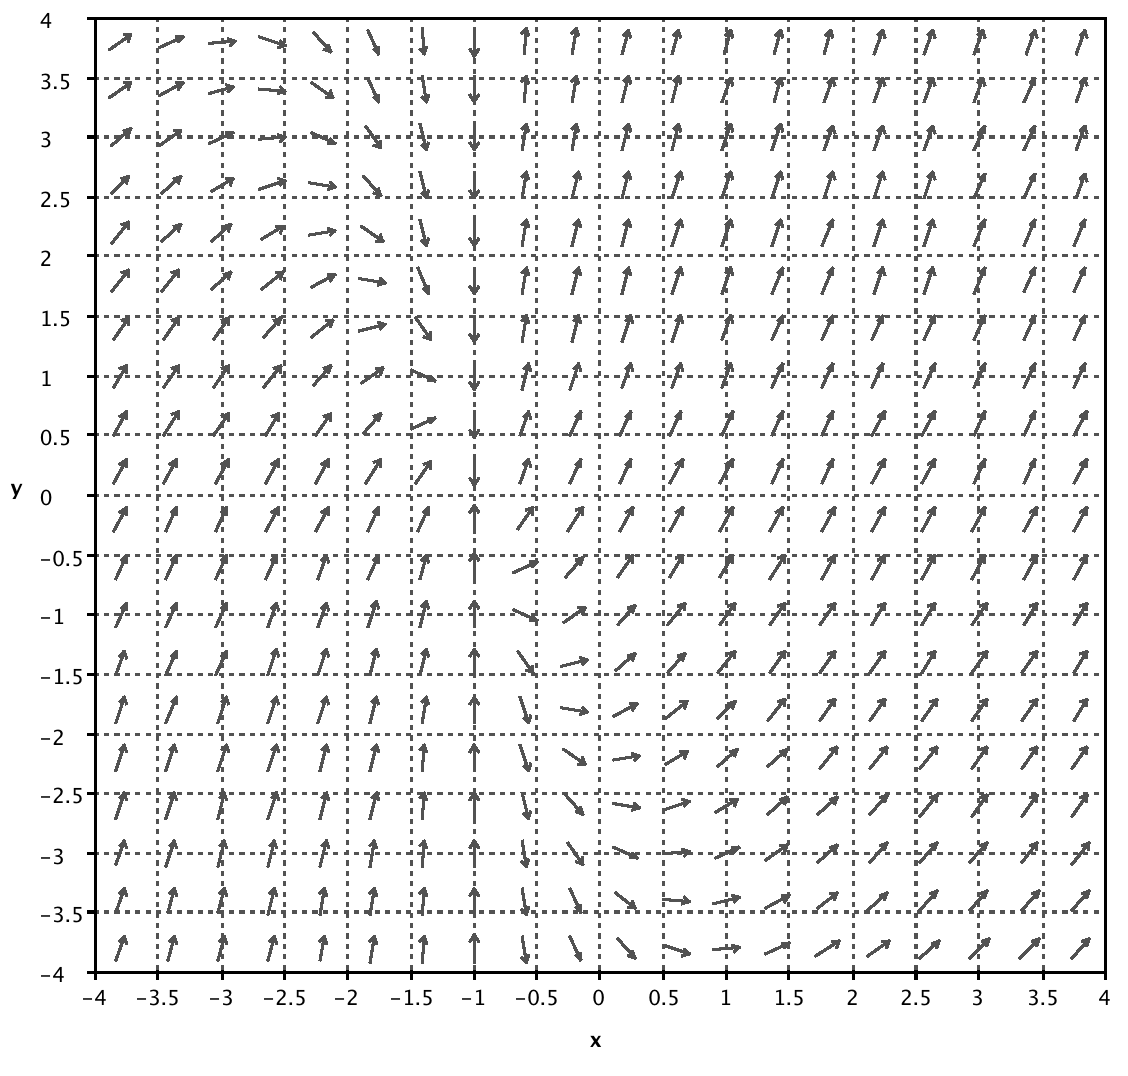
\includegraphics[scale=1]{slope.pdf}    
  % \end{center}
  \begin{center}
    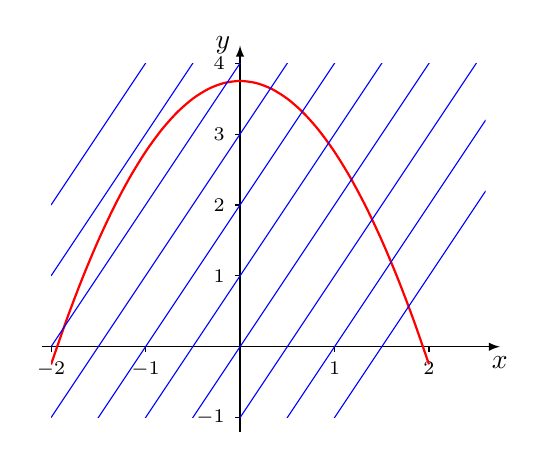
\begin{tikzpicture}[x=12mm,y=9mm,>=latex]
      \draw[thin,black,->] (-2.1,0) -- (2.75,0) node[below] {$x$};
      \draw[thin,black,->] (0,-1.2) -- (0,4.25) node[left] {$y$};
      %
      \foreach \x in {-2,-1,1,2}
      {
        \draw[thin,black] (\x,0) -- (\x,-2pt) node[below] {$\scriptstyle\x$};
      }
      \foreach \y in {-1,1,2,3,4}
      {
        \draw[thin,black] (0,\y) -- (-2pt,\y) node[left] {$\scriptstyle\y$};
      }
      \begin{scope}
        \clip (-2,-1) rectangle (2.6,4);
        \draw[thick,red,domain=-2:2,smooth] plot (\x,{3.75-(\x)^2});
        \foreach \k in {-3,-2,...,6}
        {
          \draw[thin,blue,domain=-2:2.6] plot (\x,{2*\x+\k});
        }
      \end{scope}
    \end{tikzpicture}
  \end{center}

  \alert{Question:}\ For which values of $x$ is ${\red f'(x)} > 2$?
  \begin{center}
    A\ $x<1.2$
    \quad 
    B\ $x<0$
    \quad 
    C\ $x<-1.5$
    \quad 
    D\  $x<-1$
    \quad 
    E\  $x < -0.5$
    \pause
    \quad
    \fbox{D}
  \end{center}

  % \gap Look for point on curve where curve parallel to blue line. That is the answer.


}

\frame{
  \frametitle{More Slope Questions}
  \begin{center}
    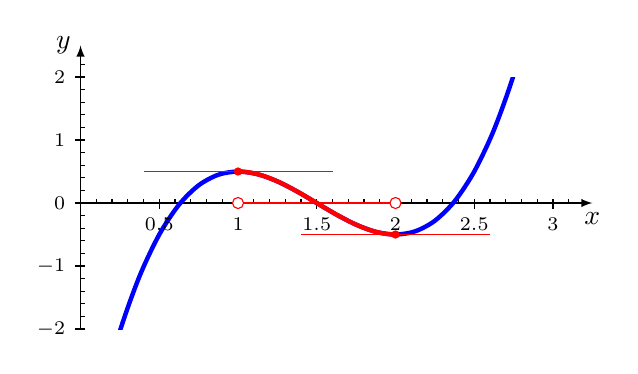
\begin{tikzpicture}[x=20mm,y=8mm,>=latex]
      \draw[thin,black,->] (0,0) -- (3.25,0) node[below] {$x$};
      \draw[thin,black,->] (0,-2) -- (0,2.5) node[left] {$y$};
      \begin{scope}
        \clip (0,-2) rectangle (3,2);
        \draw[ultra thick,blue,domain=0:3,smooth] plot (\x,{2*(\x)^3-9*(\x)^2+12*\x-4.5});
      \end{scope}
      \foreach \x in {0.5,1,1.5,2,2.5,3}
      {
        \draw[thin,black] (\x,0) -- (\x,-2pt) node[below] {$\scriptstyle\x$};
      }
      \foreach \y in {-2,-1,0,1,2}
      {
        \draw[thin,black] (0,\y) -- (-2pt,\y) node[left] {$\scriptstyle\y$};
      }
      \foreach \x in {0,0.1,...,3.15}
      {
        \draw[thin,black] (\x,0) -- (\x,1.5pt);
      }
      \foreach \y in {-2,-1.8,...,2.3}
      {
        \draw[thin,black] (0,\y) -- (1.5pt,\y);
      }
      \uncover<2>{%
        \fill[red] (1,0) circle (1.5pt);
        \fill[red] (1,0.5) circle (1.5pt);
        \fill[red] (2,0) circle (1.5pt);
        \fill[red] (2,-0.5) circle (1.5pt);
        \draw[thin,red] (0.4,0.5) -- (1.6,0.5);
        \draw[thin,red] (1.4,-0.5) -- (2.6,-0.5);
      }
      \uncover<4>{%
        \draw[thick,red] (1,0) -- (2,0);
        \draw[red,fill=white] (1,0) circle (2pt);
        \draw[red,fill=white] (2,0) circle (2pt);
        \draw[ultra thick,red,domain=1:2,smooth] plot (\x,{2*(\x)^3-9*(\x)^2+12*\x-4.5});
      }
    \end{tikzpicture}
  \end{center}

  {\red(1)}\ For which values of $x$ is $f'(x)=0$?
  \begin{center}
    A$=\text{none}$
    \quad 
    B$=\{0.63,\ 1.5, 2.38\}$
    \quad 
    C$=1$
    \quad 
    D$=\{1,2\}$
    \quad 
    E$=2$
    \pause
    \quad
    \uncover<2->{\fbox{D}}
  \end{center}
  \pause

  \uncover<3->{%
    {\red(2)}\ For which values of $x$ is $\red f'(x)<0$?
    \begin{center}
      A $x<0.63$\quad B $x<1$\quad C $1<x<2$\quad D $1.5<x<2.38$ \quad E none
      \uncover<4->{\fbox{C}}
    \end{center}
  }
}

\frame{
  \frametitle{That's it. Thanks for being here. }

  \begin{center}
    
\includegraphics[scale=.25]{Lecture 10 Picture.jpg}
  \end{center}
}








\end{document}


